\documentclass[a4paper, 12pt]{article}

\usepackage{multirow}
\usepackage[table,xcdraw]{xcolor}
\usepackage{enumerate}
\usepackage{graphicx}
\usepackage[T5]{fontenc}
\usepackage[utf8]{inputenc}
\usepackage[margin = 2cm]{geometry}
\usepackage{amsfonts, amsmath, amssymb}
\usepackage[none]{hyphenat}
\usepackage{fancyhdr}
\usepackage{float}
\usepackage{hyperref}
\usepackage{caption}
\usepackage[nottoc, notlot, notlof]{tocbibind}

\captionsetup[table]{skip=5pt}
\pagestyle{fancy}
\fancyhead[L]{Trường Đại học Khoa học Tự nhiên - ĐHQG TP.HCM}
\fancyhead[R]{Nhóm Just $4^{th}$}

\begin{document}

\begin{titlepage}
	\begin{center}
		\vspace*{1cm}
		\Large\textbf{Báo cáo \#3\\Giao diện người dùng \& Kiểm thử}\\

		\vfill
		\line(1,0){450}\\[4mm]
		\LARGE\textbf{\MakeUppercase{Dự án quản lý tạp chiếu phim}}\\[3mm]
		\Large{Nhập môn Công nghệ phần mềm (CSC13002)}\\[3mm]
		\Large{Nhóm Just $4^{th}$}
		\line(1,0){430}\\
		\vfill

		\vfill
		TP Hồ Chí Minh, ngày 09/12/2020
	\end{center}
\end{titlepage}

\tableofcontents
\thispagestyle{empty}
\clearpage

\section{Thông tin nhóm}
\label{sec:info}
\begin{enumerate}
	\item \textbf{Đường link GitHub}: \url{https://github.com/baolongnguyenmac/CinemaManagementSystem}
	\item \textbf{Đường link Trello}: \url{https://trello.com/b/OmRBLunD/báo-cáo-giao-diện-kiểm-thử}
	\item \textbf{Danh sách thành viên}
	\begin{table}[H]
		\begin{center}
			\begin{tabular}{|c|c|l|c|c|}
				\hline
				STT & MSSV     & \multicolumn{1}{c|}{Họ tên} & Email                         & SĐT        \\ \hline
				1   & 18120201 & Nguyễn Bảo Long             & 18120201@student.hcmus.edu.vn & 0919070940 \\ \hline
				2   & 18120211 & Võ Thế Minh                 & 18120211@student.hcmus.edu.vn & 0981850699 \\ \hline
				3   & 18120227 & Phạm Văn Minh Phương        & 18120227@student.hcmus.edu.vn & 0343049359 \\ \hline
				4   & 18120210 & Phạm Tống Bình Minh         & 18120210@student.hcmus.edu.vn & 0971877781 \\ \hline
				5   & 18120264 & Nguyễn Duy Vũ               & 18120264@student.hcmus.edu.vn & 0911572108 \\ \hline
			\end{tabular}
			\caption{Bảng danh sách thành viên nhóm}
		\end{center}
	\end{table}
\end{enumerate}
\clearpage

\section{Lịch sử cập nhật}
\label{sec:history}
\begin{table}[h]
	\begin{center}
		\begin{tabular}{|c|c|c|l|l|}
			\hline
			STT &Ngày cập nhật &Phiên bản &\multicolumn{1}{c|}{Mô tả chi tiết} &\multicolumn{1}{c|}{Tác giả} \\ \hline
			1 &09/12/2020 &1.0 &\begin{tabular}[c]{@{}l@{}}- Lên kế hoach test\\- Lập bộ test\\- Đặc tả testcase\end{tabular} &\begin{tabular}[c]{@{}l@{}}Phạm Tống Bình Minh\\ Nguyễn Duy Vũ\end{tabular} \\ \hline
			2 &10/12/2020 &1.1 &\begin{tabular}[c]{@{}l@{}}- Vẽ sơ đồ điều hướng giữa các\\ màn hình\\- Đặc tả giao diện\\ - Cập nhật kế hoạch làm việc\\\end{tabular} &\begin{tabular}[c]{@{}l@{}}Phạm Văn Minh Phương\\ Nguyễn Bảo Long \\ Võ Thế Minh\end{tabular} \\ \hline
			3 &12/12/2020 &1.2 &\begin{tabular}[c]{@{}l@{}}- Quản trị dự án và kế hoạch \\làm việc\end{tabular} &\begin{tabular}[c]{@{}l@{}}Nguyễn Bảo Long\end{tabular} \\ \hline
			% 4 &30/10/2020 &1.3 &- Đặc tả giao diện người dùng &Phạm Văn Minh Phương \\ \hline
			% 5 &31/10/2020 &1.5 &- Phân tích đóng góp cá nhân &Phạm Văn Minh Phương \\ \hline
		\end{tabular}
		\caption{Bảng lịch sử cập nhật các phiên bản của báo cáo yêu cầu}
	\end{center}
\end{table}
\clearpage

\section{Phân tích đóng góp cá nhân}
\label{sec:analys}
\begin{table}[H]
	\begin{center}
		\begin{tabular}{|c|l|l|c|}
			\hline
			STT & \multicolumn{1}{c|}{Họ tên} & \multicolumn{1}{c|}{Công việc tham gia}                                                & Phần trăm đóng góp \\ \hline
			1 & Nguyễn Bảo Long      & \begin{tabular}[c]{@{}l@{}}- Tổng hợp báo cáo\\- Đặc tả giao diện \\- Thiết kế front-end hệ thống\\\end{tabular}              & 20\% \\ \hline
			2 & Phạm Văn Minh Phương & \begin{tabular}[c]{@{}l@{}}- Đặc tả giao diện\\ - Vẽ sơ đồ điều hướng giữa các màn hình\\- Thiết kế front-end hệ thống\\\end{tabular}                          & 20\% \\ \hline
			3 & Võ Thế Minh          & \begin{tabular}[c]{@{}l@{}}- Vẽ biểu đồ Gantt\\ - Thiết kế bản demo back-end hệ thống\end{tabular} & 20\%               \\ \hline
			4 & Phạm Tống Bình Minh  & \begin{tabular}[c]{@{}l@{}}- Thiết kế back-end hệ thống \\- Đặc tả testcase\\- Lập bộ test\\\end{tabular}               & 20\% \\ \hline
			5 & Nguyễn Duy Vũ        & \begin{tabular}[c]{@{}l@{}}- Lên kế hoạch test\\ - Đặc tả testcase\end{tabular} & 20\% \\ \hline
		\end{tabular}
		\caption{Bảng phân tích đóng góp cá nhân}
	\end{center}
\end{table}
\clearpage

\section{Thiết kế giao diện người dùng}

\subsection{Sơ đồ và điều hướng giữa các màn hình}

\begin{itemize}
	\item Sơ đồ điều hướng màn hình
		\begin{figure}[H]
			\begin{center}
				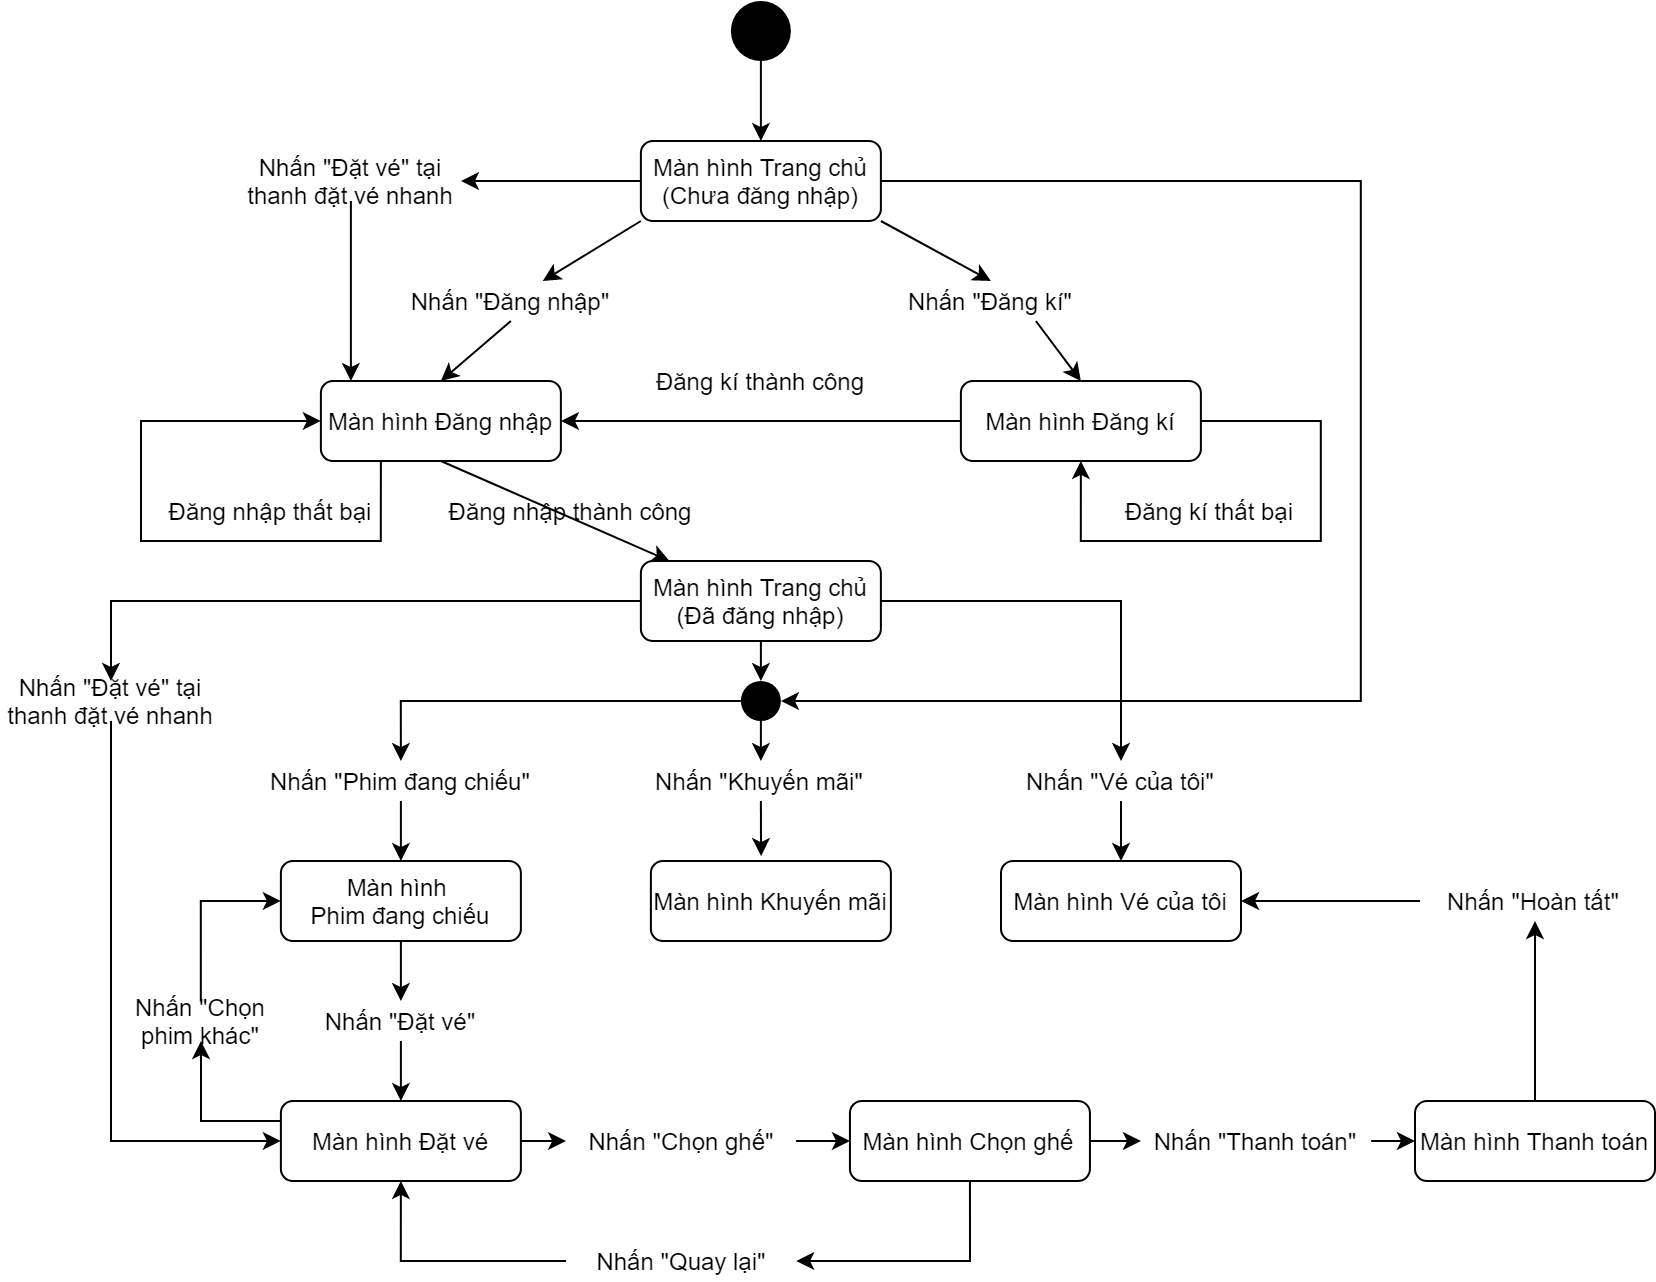
\includegraphics[scale = 0.3]{Diagram/User Screen-flow diagram.png}
				\caption{Sơ đồ điều hướng màn hình người dùng}
			\end{center}
		\end{figure}

	\clearpage

	\item Mô tả màn hình 
	\begin{table}[H]
		\begin{center}
			\begin{tabular}{|c|c|l|}
			\hline
			STT &Tên màn hình &\multicolumn{1}{c|}{Ý nghĩa/Ghi chú} \\ \hline
			1 &Trang chủ &\begin{tabular}[c]{@{}l@{}}Nơi người dùng sẽ truy cập đầu tiên. Từ đây, người dùng có thể \\ chuyển qua các màn hình Đăng nhập/Đăng kí/Phim đang chiếu\\ /Khuyến mãi/Đặt vé\end{tabular} \\ \hline
			2 &Đăng nhập &\begin{tabular}[c]{@{}l@{}}Nơi người dùng đăng nhập. Sau khi đăng nhập thành công sẽ \\ chuyển về trang chủ\end{tabular} \\ \hline
			3 &Đăng kí &Nơi người dùng đăng kí tài khoản \\ \hline
			4 &Phim đang chiếu &\begin{tabular}[c]{@{}l@{}}Hiển thị danh sách phim đang chiếu và chuyển qua màn hình \\ Đặt vé.\\ Có thể chuyển qua các màn hình khác thông qua navigation bar.\end{tabular} \\ \hline
			5 &Khuyến mãi &\begin{tabular}[c]{@{}l@{}}Hiển thị danh sách khuyến mãi.\\ Có thể chuyển qua các màn hình khác thông qua navigation bar.\end{tabular} \\ \hline
			6 &Vé của tôi &\begin{tabular}[c]{@{}l@{}}Hiển thị danh sách vé đã đặt và giao diện hủy vé.\\ Có thể chuyển qua các màn hình khác thông qua navigation bar.\end{tabular} \\ \hline
			7 &Đặt vé &\begin{tabular}[c]{@{}l@{}}Hiển thị giao diện đặt vé, có thể chuyển qua màn hình Chọn ghế.\\ Có thể chuyển qua các màn hình khác thông qua navigation bar.\end{tabular} \\ \hline
			8 &Chọn ghế &\begin{tabular}[c]{@{}l@{}}Hiển thị giao diện chọn ghế xem phim, có thể chuyển về màn hình\\ Đặt vé, chuyển qua màn hình Thanh toán.\\ Có thể chuyển qua các màn hình khác thông qua navigation bar.\end{tabular} \\ \hline
			9 &Thanh toán &\begin{tabular}[c]{@{}l@{}}Hiển thị thông tin thanh toán, có thể chuyển về màn hình Chọn ghế.\\ Có thể chuyển qua các màn hình khác thông qua navigation bar.\end{tabular} \\ \hline
			\end{tabular}
			\caption{Bảng mô tả màn hình}
		\end{center}
	\end{table}
\end{itemize}

\subsection{Đặc tả màn hình giao diện}

\subsubsection{Màn hình 1: Trang chủ}

\begin{figure}[H]
	\begin{center}
		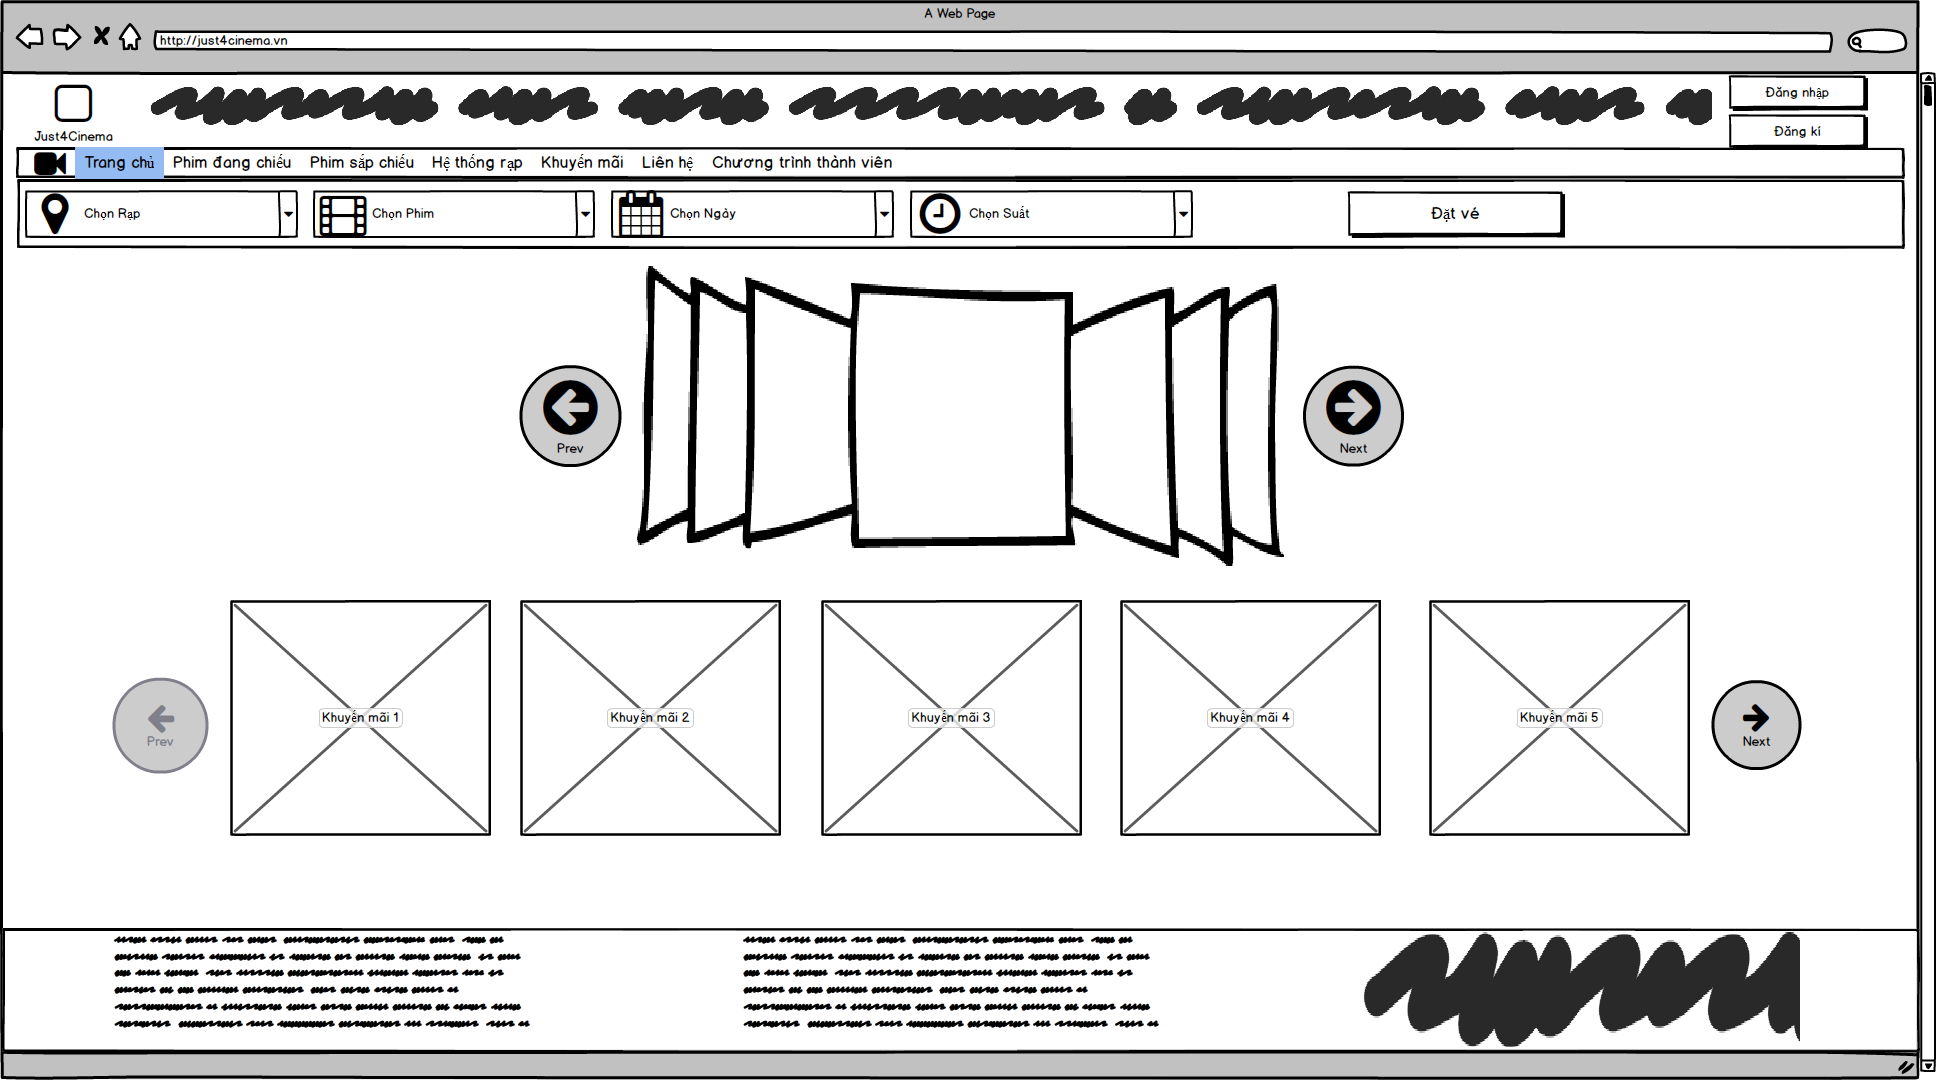
\includegraphics[scale = 0.25]{Wireframe/User/Homepage.png}
		\caption{Màn hình trang chủ}
	\end{center}
\end{figure}

\begin{itemize}
	\item Các thành phần chính
	\begin{itemize}
		\item Navigation bar
		\item Thanh "Đặt vé" nhanh
		\item Nút "Đăng nhập", "Đăng kí"
		\item Slideshow danh sách các phim đang chiếu, danh sách các khuyến mãi đang có hiệu lực
	\end{itemize}

	\item Xử lý các event trên màn hình
	\begin{itemize}
		\item Event click vào các nút trên Navigation bar, nút "Đăng nhập", nút "Đăng kí": Chuyển qua màn hình tương ứng với tên nút
		\item Event click vào nút "Đặt vé" trên thanh đặt vé nhanh: Nếu chưa chọn các thông tin về rạp, phim, suất chiếu thì hiện popup nhắc điền thông tin. Nếu đã chọn đủ các thông tin thì chuyển qua màn hình "Đặt vé"
		\item Event click vào nút mũi tên của slideshow của danh sách phim đang chiếu/khuyến mãi: Chuyển slide theo hướng mũi tên
	\end{itemize}
\end{itemize}

\subsubsection{Màn hình 2: Phim đang chiếu/Chọn phim (Trạng thái chưa đăng nhập)}

\begin{figure}[H]
	\begin{center}
		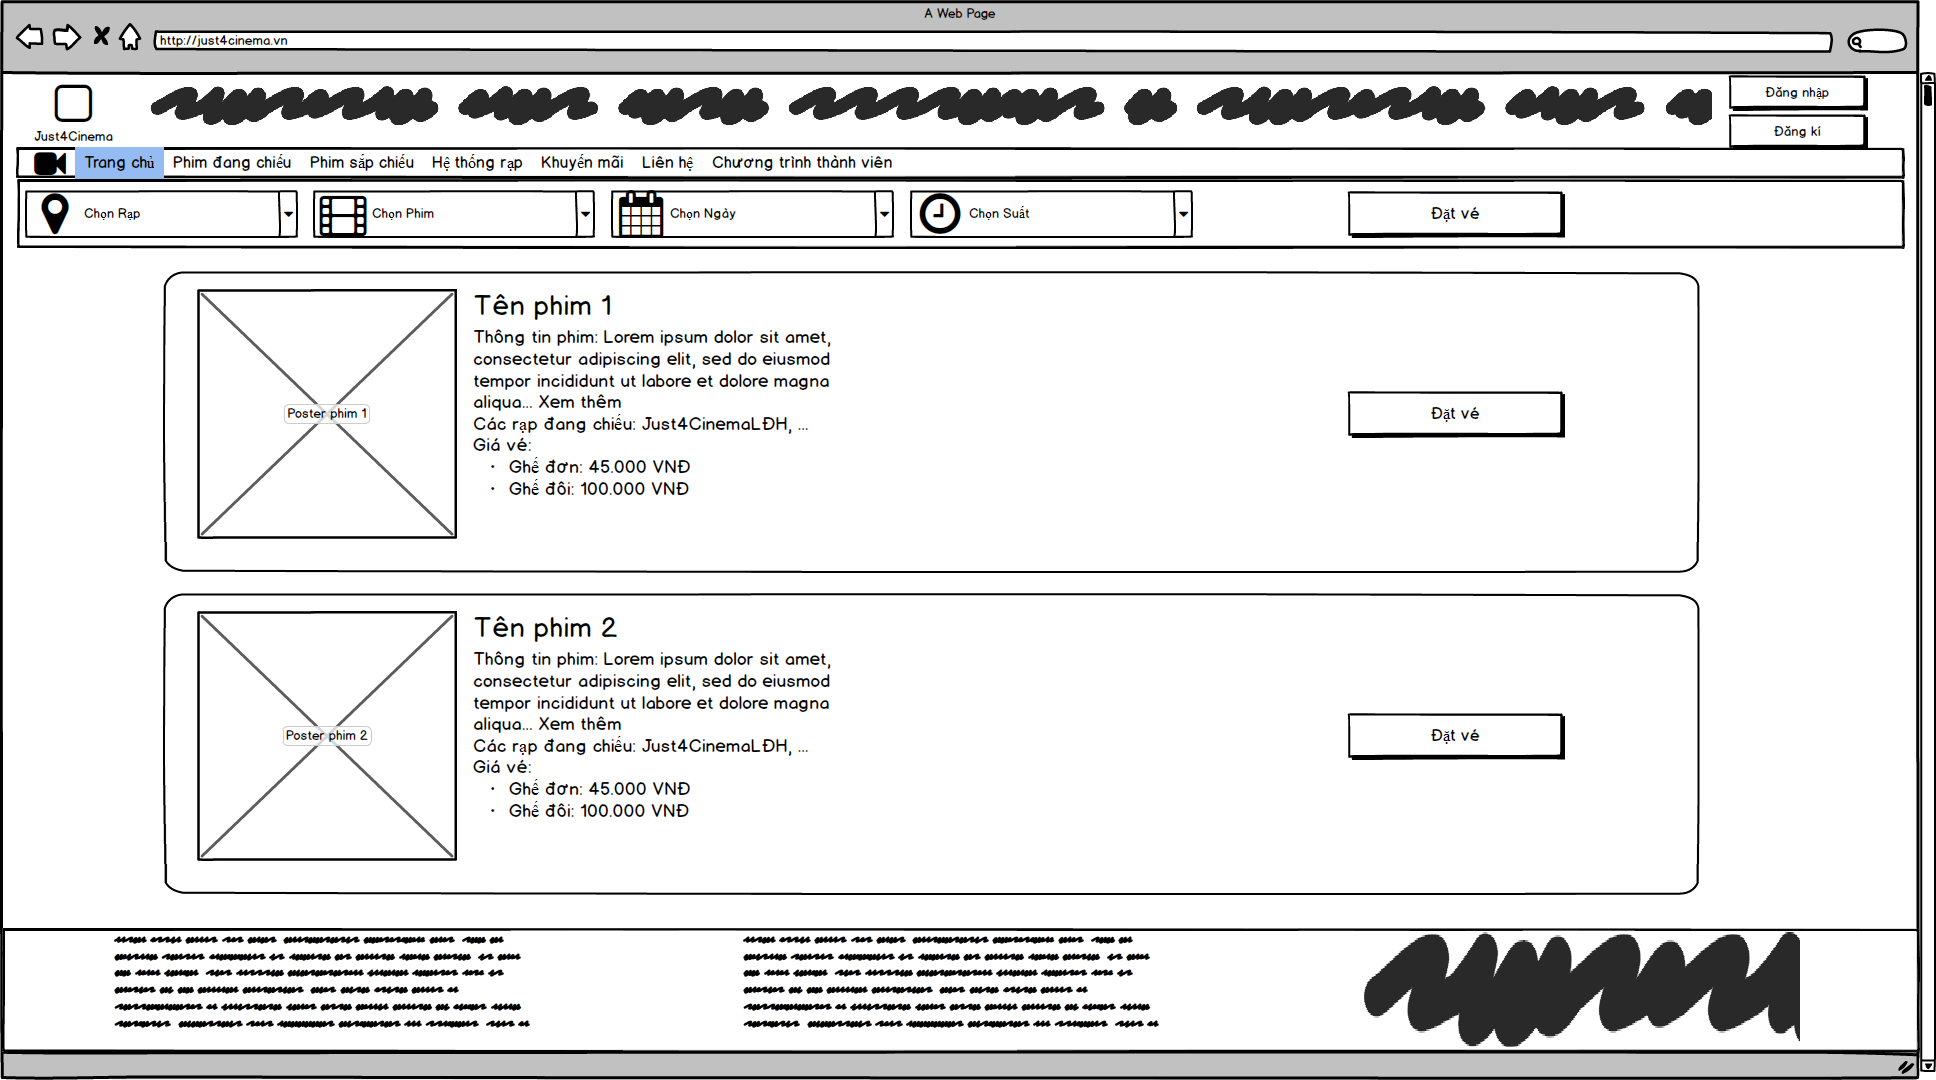
\includegraphics[scale = 0.25]{Wireframe/User/Phim đang chiếu_ Chọn phim.png}
		\caption{Màn hình phim đang chiếu/Chọn phim}
	\end{center}
\end{figure}

\begin{itemize}
	\item Các thành phần chính
	\begin{itemize}
		\item Navigation bar
		\item Thanh "Đặt vé" nhanh
		\item Nút "Đăng nhập", "Đăng kí"
		\item Danh sách các phim đang chiếu cùng nút "Đặt vé"
	\end{itemize}

	\item Xử lý các event trên màn hình
	\begin{itemize}
		\item Event click vào các nút trên Navigation bar, nút "Đăng nhập", nút "Đăng kí": Chuyển qua màn hình tương ứng với tên nút
		\item Event click vào nút "Đặt vé" trên thanh đặt vé nhanh: Nếu chưa chọn các thông tin về rạp, phim, suất chiếu thì hiện popup nhắc điền thông tin. Nếu đã chọn đủ các thông tin thì chuyển qua màn hình "Đặt vé"
		\item Event click vào nút "Đặt vé" trên danh sách phim. Nếu chưa chọn các thông tin về rạp, phim, suất chiếu thì hiện popup nhắc điền thông tin. Nếu đã chọn đủ các thông tin thì chuyển qua màn hình "Đặt vé"
	\end{itemize}
\end{itemize}

\subsubsection{Màn hình 3: Đặt vé}

\begin{figure}[H]
	\begin{center}
		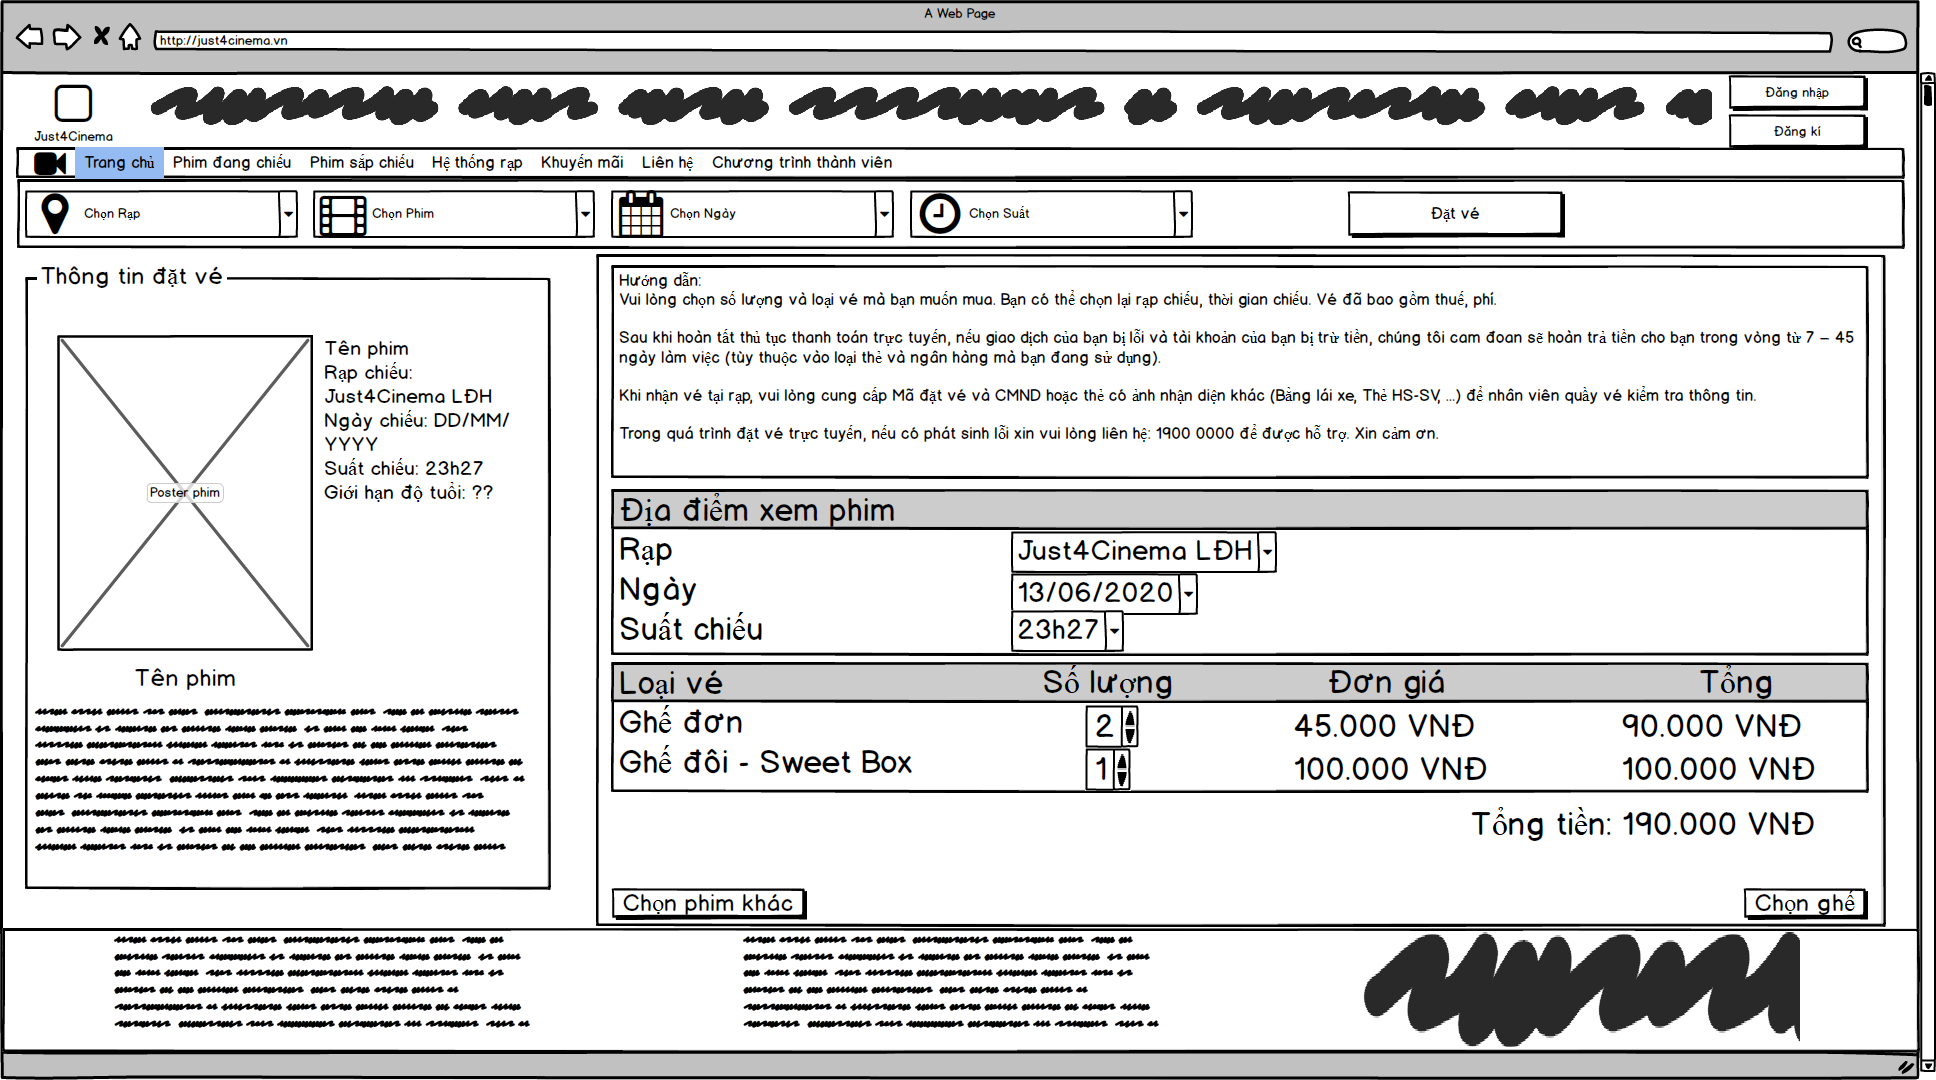
\includegraphics[scale = 0.25]{Wireframe/User/Đặt vé.png}
		\caption{Màn hình Đặt vé}
	\end{center}
\end{figure}

\begin{itemize}
	\item Các thành phần chính
	\begin{itemize}
		\item Navigation bar
		\item Thanh "Đặt vé" nhanh
		\item Nút "Đăng xuất", "Vé của tôi"
		\item Trường thông tin về vé đang đặt
		\item Các combo box, input field cho phép người dùng chỉnh sửa lại thông tin về rạp, phim, suất chiếu.
	\end{itemize}

	\item Xử lý các event trên màn hình
	\begin{itemize}
		\item Event click vào các nút trên Navigation bar, nút "Đăng nhập", nút "Đăng kí": Chuyển qua màn hình tương ứng với tên nút
		\item Event click vào nút "Đặt vé" trên thanh đặt vé nhanh: Nếu chưa chọn các thông tin về rạp, phim, suất chiếu thì hiện popup nhắc điền thông tin. Nếu đã chọn đủ các thông tin thì reload màn hình "Đặt vé" với thông tin mới chọn về rạp, phim, suất chiếu
		\item Event click vào các combo box: Đổ ra thông tin tương ứng với nhãn cho người dùng chọn
		\item Event click vào nút "Chọn ghế": Gửi thông tin vé về server, tạo yêu cầu phát sinh vé, chuyển qua màn hình "Chọn ghế"
		\item Event click vào nút "Chọn phim khác": Chuyển về màn hình "Phim đang chiếu"
	\end{itemize}
\end{itemize}

\subsubsection{Màn hình 4: Chọn ghế}

\begin{figure}[H]
	\begin{center}
		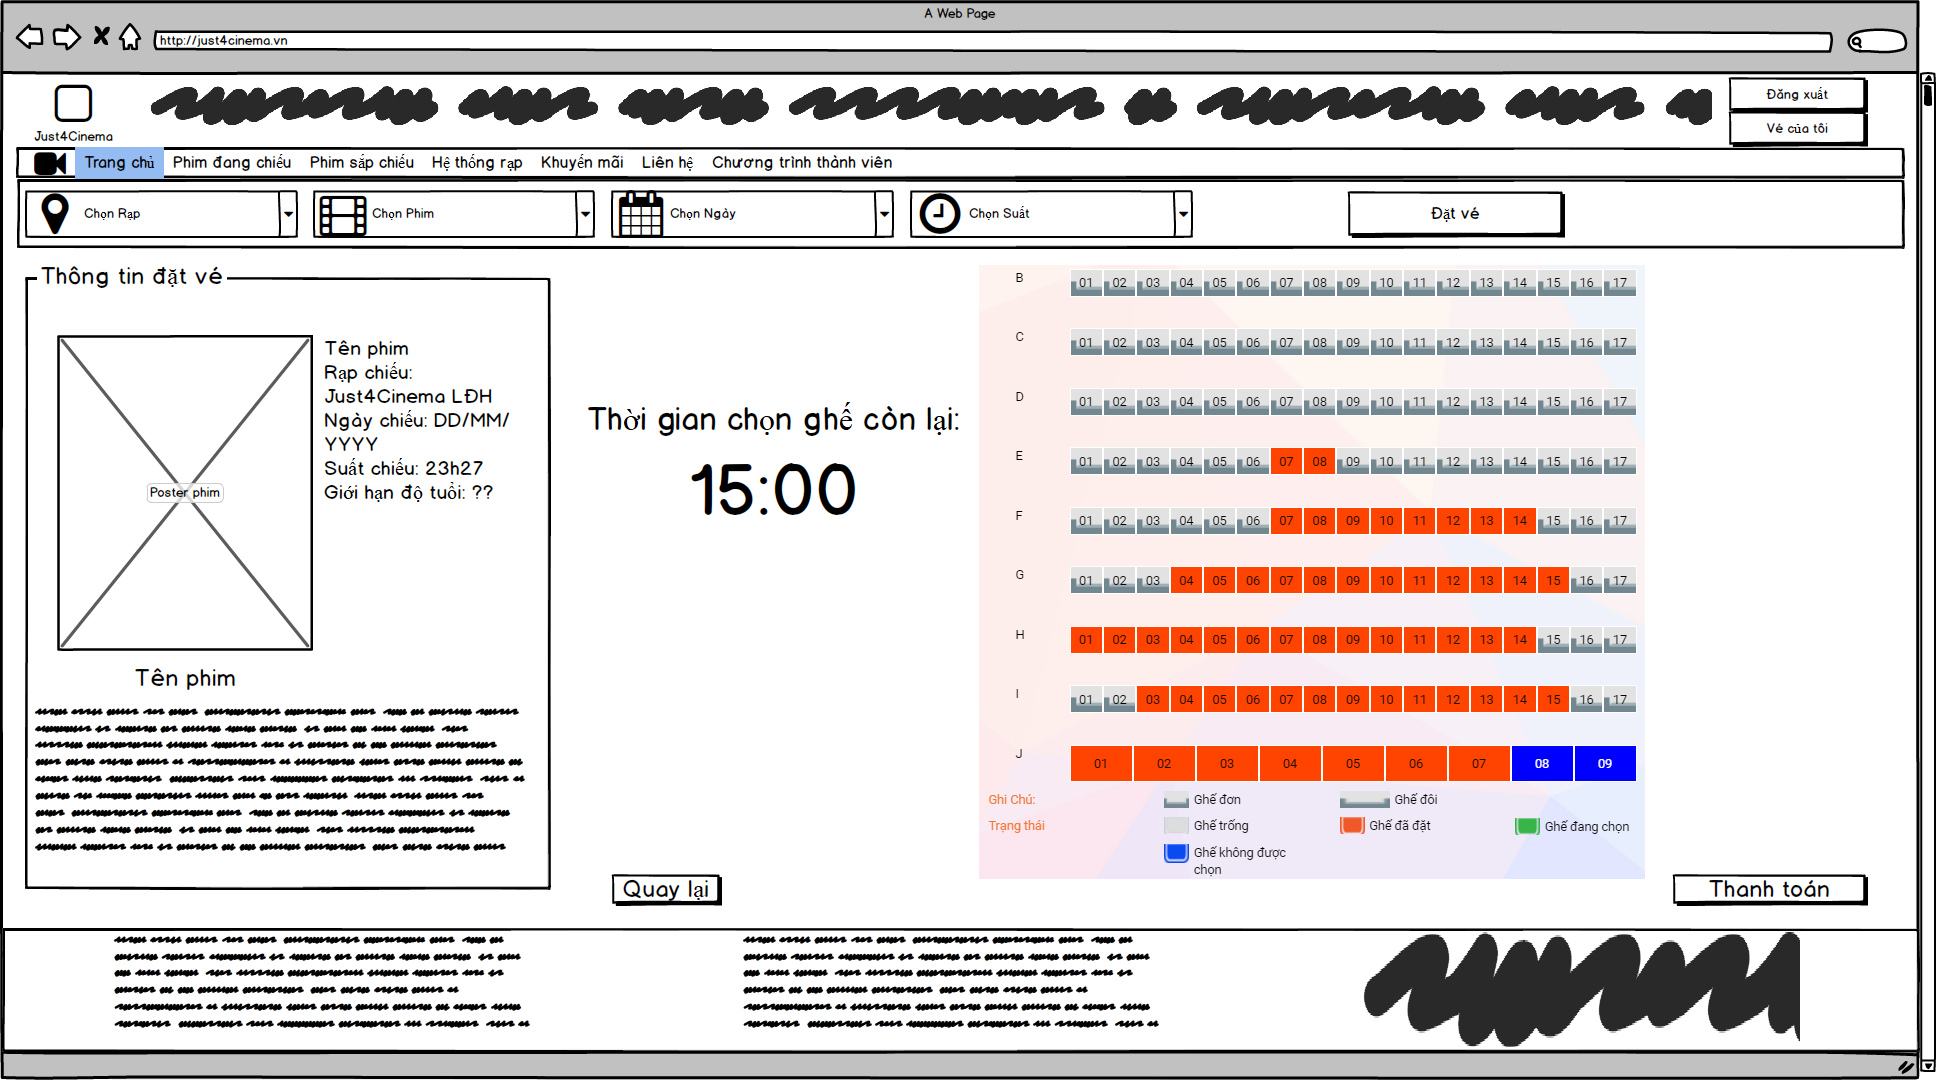
\includegraphics[scale = 0.25]{Wireframe/User/Chọn ghế.png}
		\caption{Màn hình Chọn ghế}
	\end{center}
\end{figure}

\begin{itemize}
	\item Các thành phần chính
	\begin{itemize}
		\item Navigation bar
		\item Thanh "Đặt vé" nhanh
		\item Nút "Đăng xuất", "Vé của tôi"
		\item Trường thông tin về vé đang đặt
		\item Trường chọn ghế
		\item Đồng hồ chỉ thời gian chọn ghế còn lại
	\end{itemize}

	\item Xử lý các event trên màn hình
	\begin{itemize}
		\item Event click vào các nút trên Navigation bar, nút "Đăng nhập", nút "Đăng kí": Chuyển qua màn hình tương ứng với tên nút
		\item Event click vào nút "Đặt vé" trên thanh đặt vé nhanh: Nếu chưa chọn các thông tin về rạp, phim, suất chiếu thì hiện popup nhắc điền thông tin. Nếu đã chọn đủ các thông tin thì chuyển về màn hình "Đặt vé" với thông tin mới chọn về rạp, phim, suất chiếu
		\item Event click vào các icon ghế: Đổi màu icon sang màu xanh lá cây nếu đó là ghế trống - có thể chọn
		\item Event click vào nút "Thanh toán": Gửi thông tin ghế về server, bổ sung mã ghế đã chọnvào thông tin vé, chuyển qua màn hình "Thanh toán"
		\item Event click vào nút "Quay lại": Chuyển về màn hình "Đặt vé"
	\end{itemize}
\end{itemize}

\subsubsection{Màn hình 5: Thanh toán}

\begin{figure}[H]
	\begin{center}
		\includegraphics[scale = 0.25]{Wireframe/User/Thanh toán.png}
		\caption{Màn hình Thanh toán}
	\end{center}
\end{figure}

\begin{itemize}
	\item Các thành phần chính
	\begin{itemize}
		\item Navigation bar
		\item Thanh "Đặt vé" nhanh
		\item Nút "Đăng xuất", "Vé của tôi"
		\item Trường thông tin về vé đang đặt
		\item Input field của thông tin thanh toán
		\item Trường chính sách và điều khoản thanh toán
	\end{itemize}

	\item Xử lý các event trên màn hình
	\begin{itemize}
		\item Load event: Khi màn hình được tải thì phần input field của thông tin thanh toán được điền bởi các thông tin của tài khoản khi đăng kí, có thể thay đổi.
		\item Event click vào các nút trên Navigation bar, nút "Đăng nhập", nút "Đăng kí": Chuyển qua màn hình tương ứng với tên nút
		\item Event click vào nút "Đặt vé" trên thanh đặt vé nhanh: Nếu chưa chọn các thông tin về rạp, phim, suất chiếu thì hiện popup nhắc điền thông tin. Nếu đã chọn đủ các thông tin thì chuyển về màn hình "Đặt vé" với thông tin mới chọn về rạp, phim, suất chiếu
		\item Event click vào các combo box: Đổ ra thông tin tương ứng với nhãn cho người dùng chọn
		\item Event click vào nút "Thanh toán qua Momo": Lưu thông tin thanh toán, gọi API của Momo Service, hỗ trợ thanh toán qua quét mã QR. Reload màn hình với mã QR được sinh ra từ API, yêu cầu người dùng quét để hoàn thành giao dịch.
		\item Event click vào nút "Quay lại": Chuyển về màn hình "Chọn ghế"
	\end{itemize}
\end{itemize}

\clearpage

\section{Kiểm thử phần mềm}

\subsection{Kế hoạch kiểm thử}

\begin{itemize}
	\item Nhóm Just $4^{th}$ tiến hành kiểm thử hệ thống với 2 kỹ thuật 
	\begin{itemize}
		\item Kiểm thử chức năng
		\item Kiểm thử giao diện 
	\end{itemize}

	\item Chiến thuật kiểm thử được sử dụng: Kiểm thử dựa vào chỉ dẫn
	\item Cách tiến hành
	\begin{itemize}
		\item Khi một chức năng nào đó được hoàn thành, hoạt động kiểm thử sẽ được diễn ra trên chức năng đó để đảm bảo chức năng hoạt động tốt sau đó mới được tích hợp vào hệ thống vào tiến hành kiểm thử hệ thống
		\item Sau khi được tích hợp vào hệ thống, hoạt động kiểm thử trên hệ thống sẽ được diễn ra để đảm bảo các chức năng được cài đặt trước đó hoạt động tốt sau khi tích hợp
		\item Sau cùng, tiến hành kiểm thử giao diện để đảm bảo sự hợp lý của giao diện cho người sử dụng 
	\end{itemize}
\end{itemize}

\subsection{Test case}

\subsubsection{Danh sách test case}

\begin{itemize}
	\item Chức năng Đăng ký
	\begin{table}[H]
		\centering
		\begin{tabular}{|c|c|c|l|} 
		\hline
		STT & Tên test case & \multicolumn{1}{c|}{Đối tượng test}                                           & \multicolumn{1}{c|}{Ý nghĩa}                                                                                                       \\ 
		\hline
		1   & Test case 1   & Đăng ký                                                                       & Kiểm tra trường hợp đăng ký thành công                                                                                             \\ 
		\hline
		2  & Test case 2  & Đăng ký                                                                       & \begin{tabular}[c]{@{}l@{}}Kiểm tra trường hợp đăng ký nhưng không điền đầy \\đủ thông tin \end{tabular}                           \\ 
		\hline
		3  & Test case 3  & Đăng ký                                                                       & \begin{tabular}[c]{@{}l@{}}Kiểm tra trường hợp đăng ký nhưng tài khoản đã tồn \\tại trong hệ thống \end{tabular}                   \\ 
		\hline
		\end{tabular}
		\caption{Bảng test case chức năng Đăng ký}
	\end{table}

	\item Chức năng Đăng nhập 
	\begin{table}[H]
		\centering
		\begin{tabular}{|c|c|c|l|} 
		\hline
		STT & Tên test case & \multicolumn{1}{c|}{Đối tượng test}                                           & \multicolumn{1}{c|}{Ý nghĩa}                                                                                                       \\ 
		\hline
		1   & Test case 4   & Đăng nhập                                                                     & Kiểm tra trường hợp đăng nhập thành công                                                                                           \\ 
		\hline
		3  & Test case 5  & Đăng nhập                                                                     & \begin{tabular}[c]{@{}l@{}}Kiểm tra trường hợp đăng nhập nhưng không điền \\“Tài khoản” \end{tabular}                              \\ 
		\hline
		4  & Test case 6  & Đăng nhập                                                                     & \begin{tabular}[c]{@{}l@{}}Kiểm tra trường hợp đăng nhập nhưng không điền \\“Mật khẩu” \end{tabular}                               \\ 
		\hline
		5  & Test case 7  & Đăng nhập                                                                     & \begin{tabular}[c]{@{}l@{}}Kiểm tra trường hợp đăng nhập với “Tài khoản” không \\tồn tại trong hệ thống \end{tabular}              \\ 
		\hline
		6  & Test case 8  & Đăng nhập                                                                     & Kiểm tra trường hợp đăng nhập với “Mật khẩu” sai                                                                                   \\ 
		\hline
		\end{tabular}
		\caption{Bảng test case chức năng Đăng nhập}
	\end{table}

	\item Chức năng Đăng xuất 
	\begin{table}[H]
		\centering
		\begin{tabular}{|c|c|c|l|} 
		\hline
		STT & Tên test case & \multicolumn{1}{c|}{Đối tượng test}                                           & \multicolumn{1}{c|}{Ý nghĩa}                                                                                                       \\ 
		\hline
		1   & Test case 9   & Đăng xuất                                                                     & Kiểm tra trường hợp đăng xuất thành công                                                                                           \\ 
		\hline
		\end{tabular}
		\caption{Bảng test case chức năng Đăng xuất }
	\end{table}

	\item Chức năng Đặt vé
	\begin{table}[H]
		\centering
		\begin{tabular}{|c|c|c|l|} 
		\hline
		STT & Tên test case & \multicolumn{1}{c|}{Đối tượng test}                                           & \multicolumn{1}{c|}{Ý nghĩa}                                                                                                       \\ 
		\hline
		1   & Test case 10  & Đặt vé                                                                        & Kiểm tra trường hợp đặt vé thành công                                                                                              \\ 
		\hline
		2  & Test case 11  & Đặt vé                                                                        & Kiểm tra trường hợp đặt vé nhưng chưa đăng nhập                                                                                    \\ 
		\hline
		3  & Test case 12  & Đặt vé                                                                        & Kiểm tra trường hợp đặt vé nhưng đã hết suất chiếu                                                                                 \\ 
		\hline
		4  & Test case 13  & Đặt vé                                                                        & \begin{tabular}[c]{@{}l@{}}Kiểm tra trường hợp đặt vé nhưng không điền đầy \\đủ form đặt vé \end{tabular}                          \\ 
		\hline
		5  & Test case 14  & Đặt vé                                                                        & \begin{tabular}[c]{@{}l@{}}Kiểm tra trường hợp đặt vé nhưng quá thời gian chờ \\của hệ thống \end{tabular}                         \\ 
		\hline
		\end{tabular}
		\caption{Bảng test case chức năng Đặt vé}
	\end{table}

	\item Chức năng Hủy vé 
	\begin{table}[H]
		\centering
		\begin{tabular}{|c|c|c|l|} 
		\hline
		STT & Tên test case & \multicolumn{1}{c|}{Đối tượng test}                                           & \multicolumn{1}{c|}{Ý nghĩa}                                                                                                       \\ 
		\hline
		1   & Test case 15  & Hủy vé                                                                        & Kiểm tra trường hợp hủy vé thành công                                                                                              \\ 
		\hline
		2  & Test case 16  & Hủy vé                                                                        & Kiểm tra trường hợp hủy vé nhưng chưa đăng nhập                                                                                    \\ 
		\hline
		3  & Test case 17  & Hủy vé                                                                        & Kiểm tra trường hợp hủy vé nhưng chưa mua vé                                                                                       \\ 
		\hline
		\end{tabular}
		\caption{Bảng test case chức năng Hủy vé }
	\end{table}

	\item Chức năng Thanh toán online 
	\begin{table}[H]
		\centering
		\begin{tabular}{|c|c|c|l|} 
		\hline
		STT & Tên test case & \multicolumn{1}{c|}{Đối tượng test}                                           & \multicolumn{1}{c|}{Ý nghĩa}                                                                                                       \\ 
		\hline
		1   & Test case 18  & Thanh toán online                                                             & Kiểm tra trường hợp thanh toán online thành công                                                                                   \\ 
		\hline
		2  & Test case 19  & Thanh toán online                                                             & \begin{tabular}[c]{@{}l@{}}Kiểm tra trường hợp thanh toán online nhưng nhập \\mã giảm giá sai \end{tabular}                        \\ 
		\hline
		3  & Test case 20  & Thanh toán online                                                             & \begin{tabular}[c]{@{}l@{}}Kiểm tra trường hợp thanh toán online nhưng thanh \\toán không thành công \end{tabular}                 \\ 
		\hline
		4  & Test case 21  & Thanh toán online                                                             & \begin{tabular}[c]{@{}l@{}}Kiểm tra trường hợp thanh toán online quá thời hạn \\thanh toán \end{tabular}                           \\
		\hline
		\end{tabular}
		\caption{Bảng test case chức năng Thanh toán online }
	\end{table}

	\item Chức năng Xem thông tin phim 
	\begin{table}[H]
		\centering
		\begin{tabular}{|c|c|c|l|} 
		\hline
		STT & Tên test case & \multicolumn{1}{c|}{Đối tượng test}                                           & \multicolumn{1}{c|}{Ý nghĩa}                                                                                                       \\ 
		\hline
		1   & Test case 22  & Xem thông tin phim                                                            & Kiểm tra trường hợp xem thông tin phim thành công                                                                                  \\ 
		\hline
		2  & Test case 23  & Xem thông tin phim                                                            & \begin{tabular}[c]{@{}l@{}}Kiểm tra trường hợp xem thông tin phim nhưng phim \\chưa có thông tin phim \end{tabular}                \\ 
		\hline
		\end{tabular}
		\caption{Bảng test case chức năng Xem thông tin phim }
	\end{table}

	\item Chức năng Quản lý lịch chiếu 
	\begin{table}[H]
		\centering
		\begin{tabular}{|c|c|c|l|} 
		\hline
		STT & Tên test case & \multicolumn{1}{c|}{Đối tượng test}                                           & \multicolumn{1}{c|}{Ý nghĩa}                                                                                                       \\ 
		\hline
		1   & Test case 24  & Quản lý lịch chiếu                                                            & Kiểm tra trường hợp quản lý lịch chiếu thành công                                                                                  \\ 
		\hline
		2  & Test case 25  & Quản lý lịch chiếu                                                            & \begin{tabular}[c]{@{}l@{}}Kiểm tra trường hợp quản lý lịch chiếu nhưng chỉnh \\sửa gây ra xung đột \end{tabular}                  \\ 
		\hline
		\end{tabular}
		\caption{Bảng test case chức năng Quản lý lịch chiếu }
	\end{table}

	\item Chức năng Quản lý chương trình khuyến mãi 
	\begin{table}[H]
		\centering
		\begin{tabular}{|c|c|c|l|} 
		\hline
		STT & Tên test case & \multicolumn{1}{c|}{Đối tượng test}                                           & \multicolumn{1}{c|}{Ý nghĩa}                                                                                                       \\ 
		\hline
		1   & Test case 26  & \begin{tabular}[c]{@{}l@{}}Quản lý chương \\trình khuyến mãi \end{tabular}    & \begin{tabular}[c]{@{}l@{}}Kiểm tra trường hợp quản lý chương trình khuyến \\mãi thành công \end{tabular}                          \\ 
		\hline
		2  & Test case 27  & \begin{tabular}[c]{@{}l@{}}Quản lý chương\\trình khuyến mãi \end{tabular} & \begin{tabular}[c]{@{}l@{}}Kiểm tra trường hợp quản lý các chương trình khuyến\\mãi nhưng chỉnh sửa gây ra xung đột \end{tabular}  \\ 
		\hline
		\end{tabular}
		\caption{Bảng test case chức năng Quản lý chương trình khuyến mãi }
	\end{table}

	\item Chức năng Quản lý các tài khoản của actor Quản lý 
	\begin{table}[H]
		\centering
		\begin{tabular}{|c|c|c|l|} 
		\hline
		STT & Tên test case & \multicolumn{1}{c|}{Đối tượng test}                                           & \multicolumn{1}{c|}{Ý nghĩa}                                                                                                       \\ 
		\hline
		1  & Test case 28  & \begin{tabular}[c]{@{}l@{}}Quản lý các tài \\khoản quản lý \end{tabular}      & \begin{tabular}[c]{@{}l@{}}Kiểm tra trường hợp quản lý các tài khoản quản lý \\thành công \end{tabular}                            \\ 
		\hline
		2  & Test case 29  & \begin{tabular}[c]{@{}l@{}}Quản lý các tài \\khoản quản lý \end{tabular}      & \begin{tabular}[c]{@{}l@{}}Kiểm tra trường hợp quản lý các quản lý nhưng phân\\quyền không thành công \end{tabular}                \\ 
		\hline
		\end{tabular}
		\caption{Bảng test case chức năng Quản lý các tài khoản của actor Quản lý }
	\end{table}

	\item Chức năng Thống kê doanh thu 
	\begin{table}[H]
		\centering
		\begin{tabular}{|c|c|c|l|} 
		\hline
		STT & Tên test case & \multicolumn{1}{c|}{Đối tượng test}                                           & \multicolumn{1}{c|}{Ý nghĩa}                                                                                                       \\ 
		\hline
		1  & Test case 30  & Thống kê doanh thu                                                            & Kiểm tra trường hợp thống kê doanh thu thành công                                                                                  \\ 
		\hline
		\end{tabular}
		\caption{Bảng test case chức năng Thống kê doanh thu }
	\end{table}
\end{itemize}

\clearpage 

\subsubsection{Đặc tả test case}

\begin{enumerate}
	\item Đặc tả test case Đăng ký
	\begin{table}[H]
		\centering
		\begin{tabular}{|l|l|} 
		\hline
		\multicolumn{1}{|l|}{Test case} & \multicolumn{1}{l|}{Test case 1}                                                                                                     \\ 
		\hline
		Related Use case                & Đăng ký                                                                                                                              \\ 
		\hline
		Context                         & Người dùng đăng ký thành công với “Tài khoản” và “Mật khẩu” hợp lệ                                                                   \\ 
		\hline
		Input Data                      & Tài khoản: just4thdangky                                                                                                             \\
										& Mật khẩu: 123456                                                                                                                     \\
										& Họ tên: just4th                                                                                                                      \\ 
		\hline
		Expected Output                 & \begin{tabular}[c]{@{}l@{}}Xuất hiện cửa sổ thông báo “Đăng ký thành công” và tài khoản được \\cập nhật trong hệ thống\end{tabular}  \\ 
		\hline
		Test steps                      & 1. Nhập “Tài khoản”                                                                                                                   \\
										& 2. Nhập “Mật khẩu”                                                                                                                    \\
										& 3. Nhập “Họ tên”                                                                                                                      \\
										& 4. Click nút “Đăng ký”                                                                                                                \\
		\hline
		\end{tabular}
		\caption{Bảng tóm tắt test case của hệ thống}
	\end{table}

	\item Đặc tả test case Đăng nhập
	\begin{table}[H]
		\centering
		\begin{tabular}{|l|l|} 
		\hline
		\multicolumn{1}{|l|}{Test case} & \multicolumn{1}{l|}{Test case 4}                                                                                                             \\ 
		\hline
		Related Use case                & Đăng nhập                                                                                                                                    \\ 
		\hline
		Context                         & \begin{tabular}[c]{@{}l@{}}Người dùng đăng nhập vào hệ thống thành công với tài khoản và mật\\ khẩu đã tồn tại trong hệ thống \end{tabular}  \\ 
		\hline
		Input Data                      & Tài khoản: just4thdangky                                                                                                                     \\
										& Mật khẩu: 123456                                                                                                                             \\ 
		\hline
		Expected Output                 & Xuất hiện cửa sổ thông báo “Đăng nhập thành công”                                                                                            \\ 
		\hline
		Test steps                      & 1. Nhập “Tài khoản”                                                                                                                           \\
										& 2. Nhập “Mật khẩu”                                                                                                                            \\
										& 3. Click nút “Đăng nhập”                                                                                                                      \\
		\hline
		\end{tabular}
		\caption{Bảng đặc tả test case 4}
	\end{table}

	\item Đặc tả test case Đăng xuất
	\begin{table}[H]
		\centering
		\begin{tabular}{|l|l|} 
		\hline
		\multicolumn{1}{|l|}{Test case} & \multicolumn{1}{l|}{Test case 9}                         \\ 
		\hline
		Related Use case                & Đăng xuất                                                \\ 
		\hline
		Context                         & Người dùng đăng xuất khỏi tài khoản hiện tại thành công  \\ 
		\hline
		Input Data                      & Không                                                    \\ 
		\hline
		Expected Output                 & Xuất hiện cửa sổ thông báo “Đăng xuất thành công”        \\ 
		\hline
		Test steps                      & Click nút “Đăng xuất”                                  \\
		\hline
		\end{tabular}
		\caption{Bảng đặc tả test case 9}
	\end{table}

	\clearpage

	\item Đặc tả test case Đặt vé
	\begin{table}[H]
		\centering
		\begin{tabular}{|l|l|} 
		\hline
		\multicolumn{1}{|l|}{Test case} & \multicolumn{1}{l|}{Test case 10}                                                                                                       \\ 
		\hline
		Related Use case                & Đặt vé                                                                                                                                  \\ 
		\hline
		Context                         & Người dùng đặt vé thành công                                                                                                            \\ 
		\hline
		Input Data                      & Không                                                                                                                                   \\ 
		\hline
		Expected Output                 & \begin{tabular}[c]{@{}l@{}}Xuất hiện cửa sổ thông báo “Đặt vé thành công”, thông tin đặt vé \\được cập nhật trên hệ thống\end{tabular}  \\ 
		\hline
		Test steps                      & 1. Chọn phim muốn xem                                                                                                                    \\
										& 2. Điền form đặt vé                                                                                                                      \\
										& 3. Chọn lịch chiếu, ghế                                                                                                                  \\
										& 4. Click nút “Thanh toán”                                                                                                                \\
		\hline
		\end{tabular}
		\caption{Bảng đặc tả test case 10}
	\end{table}

	\item Đặc tả test case Hủy vé
	\begin{table}[H]
		\centering
		\begin{tabular}{|l|l|} 
		\hline
		\multicolumn{1}{|l|}{Test case} & \multicolumn{1}{l|}{Test case 15}                                                                                                      \\ 
		\hline
		Related Use case                & Hủy vé                                                                                                                                 \\ 
		\hline
		Context                         & Người dùng hủy vé thành công                                                                                                           \\ 
		\hline
		Input Data                      & Không                                                                                                                                  \\ 
		\hline
		Expected Output                 & \begin{tabular}[c]{@{}l@{}}Xuất hiện cửa sổ thông báo “Hủy vé thành công”, thông tin hủy vé\\được cập nhật trên hệ thống\end{tabular}  \\ 
		\hline
		Test steps                      & 1. Chọn phim muốn xem                                                                                                                   \\
										& 2. Click nút “Hủy vé”                                                                                                                   \\
		\hline
		\end{tabular}
		\caption{Bảng đặc tả test case 15}
	\end{table}

	\item Đặc tả test case Xem thông tin phim
	\begin{table}[H]
		\centering
		\begin{tabular}{|l|l|} 
		\hline
		\multicolumn{1}{|l|}{Test case} & \multicolumn{1}{l|}{Test case 22}                \\ 
		\hline
		Related Use case                & Xem thông tin phim                               \\ 
		\hline
		Context                         & Người dùng xem thông tin phim thành công         \\ 
		\hline
		Input Data                      & Không                                            \\ 
		\hline
		Expected Output                 & Hiển thị thông tin phim của người dùng muốn xem  \\ 
		\hline
		Test steps                      & 1. Chọn phim muốn xem lịch chiếu                  \\
										& 2. Nhấn nút “Xem lịch chiếu”                      \\
		\hline
		\end{tabular}
		\caption{Bảng đặc tả test case 22}
	\end{table}

	\clearpage

	\item Đặc tả test case Thanh toán online 
	\begin{table}[H]
		\centering
		\begin{tabular}{|l|l|} 
		\hline
		\multicolumn{1}{|l|}{Test case} & \multicolumn{1}{l|}{Test case 18}                                                                                                                      \\ 
		\hline
		Related Use case                & Thanh toán online                                                                                                                                      \\ 
		\hline
		Context                         & Người dùng thanh toán online thành công                                                                                                                \\ 
		\hline
		Input Data                      & Mã giảm giá: giamgia                                                                                                                                   \\ 
		\hline
		Expected Output                 & \begin{tabular}[c]{@{}l@{}}Hiển thị cửa sổ “Thanh toán online thành công”, thông tin thanh toán thành \\công được cập nhật trên hệ thống\end{tabular}  \\ 
		\hline
		Test steps                      & 1. Nhập “Mã giảm giá”                                                                                                                                   \\
										& 2. Click nút kiểm tra mã giảm giá                                                                                                                       \\
										& 3. Nhấn nút “Tiếp tục”                                                                                                                                  \\
										& 4. Quét mã thanh toán                                                                                                                                   \\
		\hline
		\end{tabular}
		\caption{Bảng đặc tả test case 18}
	\end{table}

	\item Đặc tả test case Quản lý thông tin phim
	\begin{table}[H]
		\centering
		\begin{tabular}{|l|l|} 
		\hline
		\multicolumn{1}{|l|}{Test case} & \multicolumn{1}{l|}{Test case 24}                               \\ 
		\hline
		Related Use case                & Quản lý thông tin phim                                          \\ 
		\hline
		Context                         & Quản lý quản lý các lịch chiếu trong rạp chiếu phim thành công  \\ 
		\hline
		Input Data                      & Không                                                           \\ 
		\hline
		Expected Output                 & Hiển thị cửa sổ “Chỉnh sửa thành công”                          \\ 
		\hline
		Test steps                      & 1. Chọn phim muốn chỉnh sửa                                      \\
										& 2. Thực hiện chỉnh sửa                                           \\
										& 3. Click nút “Hoàn tất”                                          \\
		\hline
		\end{tabular}
		\caption{Bảng đặc tả test case 24}
	\end{table}
\end{enumerate}

\clearpage

\section{Quản trị dự án và kế hoạch làm việc}

\subsection{Báo cáo tiến độ}

\begin{itemize}
	\item Các công việc đã hoàn thành
	\begin{itemize}
		\item Xác thực đặt vé, huỷ vé, quản lý thông tin phim phía back-end
		\item Giao diện chức năng đặt vé, huỷ vé
	\end{itemize}
	\item Công việc chưa hoàn thành: Giao diện chức năng quản lý thông tin phim 

	\item Tính tới thời điểm hiện tại, mọi công việc đều đang đi đúng theo tiến độ
	\item Giải pháp làm việc việc đúng tiến độ: Tận dụng thời gian để học công nghệ liên quan đến các công việc cần làm và thực hành nháp để quen với công nghệ mới sau đó bắt tay vào thực hiện công việc
\end{itemize}

\clearpage 

\subsection{Kế hoạch thực hiện}

\begin{itemize}
	\item ID của các tác vụ và các milestone được giải thích chi tiết trong báo cáo 1
	\item Biểu đồ Gantt 
	\begin{figure}[H]
		\begin{center}
			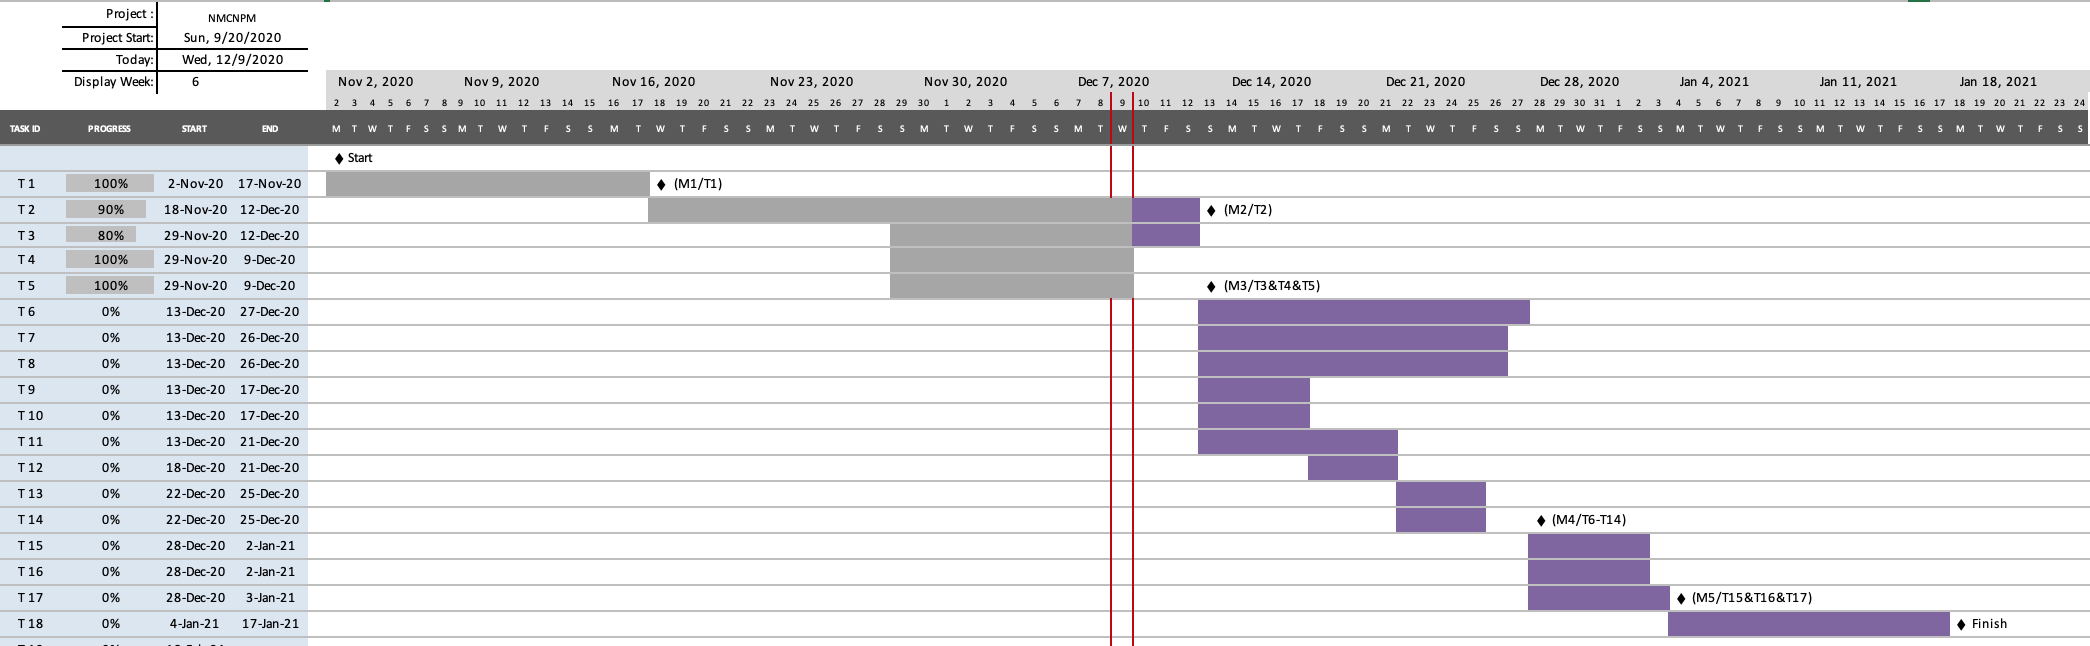
\includegraphics[scale=0.45, angle=90]{./image/gantt.png}
			\caption{Biểu đồ Gantt}
		\end{center}
	\end{figure}
\end{itemize}

\subsection{Phân rã trách nhiệm}

\begin{itemize}
	\item Từ ngày 18/11/2020 đến ngày 12/12/2020, các thành viên trong nhóm chịu trách nhiệm cho các công việc sau
	\begin{table}[H]
		\begin{center}
			\begin{tabular}{|c|l|l|}
			\hline
			STT & \multicolumn{1}{c|}{Họ tên} & \multicolumn{1}{c|}{Công việc}                         \\ \hline
			1 & \multirow{3}{*}{\begin{tabular}[c]{@{}l@{}}- Nguyễn Bảo Long\\ - Phạm Văn Minh Phương\end{tabular}} & Thiết kế giao diện chức năng Huỷ vé    \\ \cline{1-1} \cline{3-3} 
			2   &                             & Thiết kế giao diện chức năng Đặt vé                    \\ \cline{1-1} \cline{3-3} 
			3   &                             & Thiết kế giao diện chức năng Quản lý thông tin phim    \\ \hline
			4 & \multirow{3}{*}{\begin{tabular}[c]{@{}l@{}}- Võ Thế Minh\\ - Phạm Tống Bình Minh\end{tabular}}      & Thiết kế back-end cho chức năng Đặt vé \\ \cline{1-1} \cline{3-3} 
			5   &                             & Thiết kế back-end cho chức năng Huỷ vé                 \\ \cline{1-1} \cline{3-3} 
			6   &                             & Thiết kế back-end cho chức năng Quản lý thông tin phim \\ \hline
			4   & - Nguyễn Duy Vũ             & Triển khai kiểm thử                                    \\ \hline
			\end{tabular}
			\caption{Bảng phân rã trách nhiệm đối với từng công việc cụ thể}
		\end{center}
	\end{table}

	\item Thành viên điều phối việc tích hợp: Phạm Tống Bình Minh 
	\item Thành viên điều phối việc kiểm thử tích hợp: Nguyễn Duy Vũ
\end{itemize}

\clearpage

\section{Tham khảo}

\end{document}